\chapter{Design}
\section{Scope}
\section{Threat model}
\section{Security properties}
\section{Requirements}
\section{Architecture}
\begin{figure}[h]
	\centering
	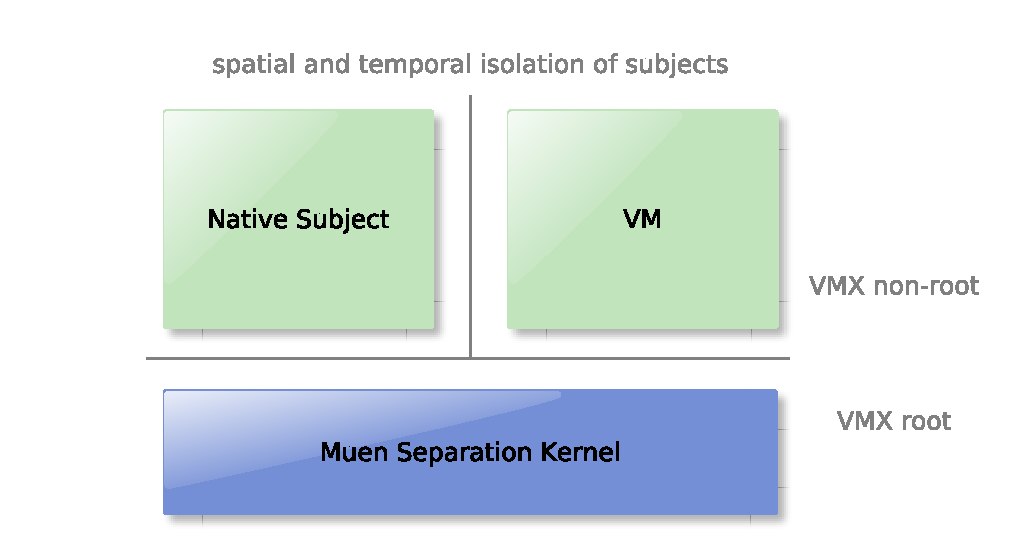
\includegraphics[scale=0.7]{images/architecture-overview}
	\caption{Architecture overview}
	\label{fig:architecture-overview}
\end{figure}

\subsection{Virtualization}
\subsection{Scheduling}\label{subsec:scheduling}
This section presents the design of the Muen kernel scheduler and the selected
scheduling algorithm.

In the context of this work, scheduling is defined as the process of selecting
a subject and giving it access to system resources for a certain amount of time.
The main resource is processor time, which enables a subject to execute and
perform its task.

A key objective of the scheduler is to provide temporal isolation of all
subjects. In order to meet this requirement, the scheduler must prevent any
interference between subjects. To achieve this, scheduling is done in a fixed,
cyclic and preemptive manner.

Subjects are executed for a fixed amount of time, before being preempted by the
scheduler. Preemption means that regardless of what operations a subject is
performing, its execution is suspended when the alloted time quantum has been
consumed. After a subject has been suspended, the scheduler executes the next
subject for a given amount of time.

The information of which subject runs for how long and the chronologic sequence
of subjects is contained in a \emph{scheduling plan}\index{Scheduling plan}.
Such a plan is part of the policy and specifies in what order subjects are
executed in which logical CPU and for how long. The task of scheduler is then to
enforce a given scheduling regime.

A scheduling plan is specified in terms of frames. A \emph{major frame}
\index{Major frame} consists of a sequence of minor frames. When the end of a
major is reached, the scheduler starts over from the beginning and uses the
first minor frame in a cyclic fashion. A \emph{minor frame}\index{Minor frame}
specifies a subject and a precise amount of time. This information is directly
applied by the scheduler.

An example scheduling plan is depicted in figure
\ref{fig:example-scheduling-plan}. It illustrated a system with two logical CPUs
that execute various subjects indicated by different colors. Since major frames
are repeated, major frame one and two are identical. All CPUs of the system
wait on a barrier at the beginning of a new major frame. This guarantees that
all logical CPUs of a system are in-sync on major frame changes.

CPU 0 is executing the same subject for the whole duration of the major frame.
This could for example be the $\tau$0 subject executing on the bootstrap
processor (BSP). The second CPU is executing two subjects (blue and green) in
alternating order. As can be seen, subject green is granted more CPU cycles than
subject blue.

\begin{figure}[ht]
	\begin{ganttchart}[
		vgrid={*9{dotted},*1{dashed},*9{dotted}},
		hgrid,
		y unit title=0.75cm,
		title label anchor/.style={below=-1.5ex}]{20}
		\gantttitle{Major frame 1}{10}
		\gantttitle{Major frame 2}{10} \\
		\ganttbar[bar/.append style={fill=Apricot}]{CPU 0}{1}{10}
		\ganttbar[bar/.append style={fill=Apricot}]{}{11}{20} \\
		\ganttbar[bar/.append style={fill=CornflowerBlue}]{CPU 1}{1}{2}
		\ganttbar[bar/.append style={fill=YellowGreen}]{}{3}{6}
		\ganttbar[bar/.append style={fill=CornflowerBlue}]{}{7}{8}
		\ganttbar[bar/.append style={fill=YellowGreen}]{}{9}{10}
		\ganttbar[bar/.append style={fill=CornflowerBlue}]{}{11}{12}
		\ganttbar[bar/.append style={fill=YellowGreen}]{}{13}{16}
		\ganttbar[bar/.append style={fill=CornflowerBlue}]{}{17}{18}
		\ganttbar[bar/.append style={fill=YellowGreen}]{}{19}{20}
	\end{ganttchart}
	\caption{Example scheduling plan}
	\label{fig:example-scheduling-plan}
\end{figure}

On systems with multiple logical CPUs, a scheduling plan must specify a sequence
of minor frames for each processor core. In order for the cores to not run out
of sync, all major frames must be of equal length. This means that the sum of
all minor frame time slices of all major frames of a given scheduling plan must
amount to the same time duration.

Figure \ref{fig:example-scheduling-plan-of-a-cpu} illustrates the scheduling
plan for a specific CPU. The major frame consists of four minor frames. Minor
frame two has twice the amount of ticks than the other minor frames, which have
identical length.

When the major frame starts, subject one is scheduled for the length of minor
frame one, followed by a switch to subject 2. After that the two subjects are
again scheduled in alternating fashion.

\begin{figure}[ht]
	\begin{ganttchart}[
		vgrid={*3{dotted},*1{dashed},*7{dotted},*1{dashed},*3{dotted},*1{dashed},*3{dotted}},
		hgrid,
		y unit title=0.75cm,
		title label anchor/.style={below=-1.5ex}]{20}
		\gantttitle{Major frame}{20} \\
		\gantttitle{Minor 1}{4}
		\gantttitle{Minor 2}{8}
		\gantttitle{Minor 3}{4}
		\gantttitle{Minor 4}{4} \\
		\ganttbar[bar/.append style={fill=CornflowerBlue}]{Subject 1}{1}{4}
		\ganttbar[bar/.append style={fill=CornflowerBlue}]{}{13}{16} \\
		\ganttbar[bar/.append style={fill=YellowGreen}]{Subject 2}{5}{12}
		\ganttbar[bar/.append style={fill=YellowGreen}]{}{17}{20}
	\end{ganttchart}
	\caption{Example scheduling plan of a CPU}
	\label{fig:example-scheduling-plan-of-a-cpu}
\end{figure}

Since a system performs diverse tasks with different resource requirements,
there is a need for some flexibility with regards to scheduling. To provide this
degree of freedom while keeping the kernel complexity low, multiple scheduling
plans can be specified in the system policy. The privileged subject $\tau$0 is
then allowed to select and activate one of these scheduling plans. The kernel
enforces the current plan designated by $\tau$0.

By defining a distinct plan for each anticipated workload at integration time,
the scheduling regimes are fixed at integration time. This removes any runtime
uncertainty that might be introduced by making this mechanism, since the
scheduling plans cannot be altered at runtime.
